
如前一节所述,编译器是一种复杂的软件。收集统计数字(例如,特定优化处理的基本块的数量)是快速了解编译器运行时行为的最简单和最有效的方法。

在LLVM中收集统计信息有几种方法。本节中,我们将学习三种最常见和有用的方法,这些方法在这里概述:

\begin{itemize}
\item 使用\texttt{Statistic}类
\item 使用优化注释
\item 添加耗时测量
\end{itemize}

第一个选项是通过简单的计数器,收集统计信息的通用工具。第二个选项是专门设计用来分析编译器优化的。最后一项,用于在编译器中收集计时信息。

从第一个开始。

\subsubsubsection{11.3.1\hspace{0.2cm}使用\texttt{Statistic}类}

本节中,我们将通过对上一节中的LLVM Pass——\texttt{SimpleMulOpt}——进行修改来演示新特性。首先,我们不仅想从乘法指令中打印出操作数\texttt{Value},而且还想计算Pass已经处理了多少乘法指令。首先,尝试使用我们刚刚了解的\texttt{LLVM\_DEBUG}基础架构来实现这个特性,如下所示:

\begin{lstlisting}[style=styleCXX]
#define DEBUG_TYPE "simple-mul-opt"
PreservedAnalyses
SimpleMulOpt::run(Function &F, FunctionAnalysisManager &FAM) {
	unsigned NumMul = 0;
	for (auto &I : instructions(F)) {
		if (auto *BinOp = dyn_cast<BinaryOperator>(&I) &&
		BinOp->getOpcode() == Instruction::Mul) {
			++NumMul;
			…
		}
	}
	LLVM_DEBUG(dbgs() << "Number of multiplication: " << NumMul);
	…
}
\end{lstlisting}

这种方法看起来非常简单。但它有一个缺点——我们感兴趣的统计数字与其他调试消息混杂在一起。我们需要采取额外的操作来解析或过滤我们想要的值,尽管可能会有读者说这些问题可以通过为每个计数器变量使用单独的DEBUG\_TYPE标签来解决,但当计数器变量的数量增加时,可能会发现自己创建了大量的冗余代码。

一个很好的解决方案是使用LLVM提供的\texttt{Statistic}类(和相关工具)。下面是使用这个解决方案重写的版本:

\begin{lstlisting}[style=styleCXX]
#include "llvm/ADT/Statistic.h"
#define DEBUG_TYPE "simple-mul-opt"
STATISTIC(NumMul, "Number of multiplications processed");
PreservedAnalyses
SimpleMulOpt::run(Function &F, FunctionAnalysisManager &FAM) {
	for (auto &I : instructions(F)) {
		if (auto *BinOp = dyn_cast<BinaryOperator>(&I) &&
		BinOp->getOpcode() == Instruction::Mul) {
			++NumMul;
			…
		}
	}
	…
}
\end{lstlisting}

前面的代码展示了\texttt{Statistic}的用法,调用\texttt{STATISTIC}宏函数来创建一个\texttt{Statistic}类型变量(带有文本描述),并像使用普通整数计数器变量一样使用即可。

这个解决方案只需要修改原始代码中的几行,而且它收集所有的计数器值,并在优化结束时将它们打印出来,例如:在\texttt{opt}中使用\texttt{-stats}标志运行\texttt{SimpleMulOpt} Pass,会得到以下输出:

\begin{tcblisting}{commandshell={}}
$ opt -stats –load-pass-plugin=… …
===-------------------------------===
      … Statistics Collected …
===-------------------------------===
87 simple-mul-opt - Number of multiplications processed
$
\end{tcblisting}

87是\texttt{SimpleMulOpt}中处理的乘法指令数。当然,可以随意添加任意数量的统计计数器,以便收集不同的统计信息。如果在管道中运行多个Pass,那么所有的统计数字都将显示在同一个表中,例如:如果在\texttt{SimpleMulOpt}中添加另一个统计计数器,以从乘法指令中收集多个常数操作数的非幂数,并运行Pass SROA,可以得到类似于下面所示的输出:

\begin{tcblisting}{commandshell={}}
$ opt -stats –load-pass-plugin=… --passes="sroa,simple-multopt" …
===-------------------------------===
       … Statistics Collected …
===-------------------------------===
94 simple-mul-opt - Number of multiplications processed
87 simple-mul-opt - Number of none-power-of-two constant
operands
100 sroa - Number of alloca partition uses rewritten
34 sroa - Number of instructions deleted
… 
$
\end{tcblisting}

前面代码中的第二列是原始Pass的名称,它由\texttt{DEBUG\_TYPE}指定,在任何调用\texttt{STATISTIC}之前定义。

或者,可以通过在\texttt{opt}中添加\texttt{-stats-json}标志来输出JSON格式的结果:

\begin{tcblisting}{commandshell={}}
$ opt -stats -stats-json –load-pass-plugin=… …
{
  "simple-mul-opt.NumMul": 87
}
$
\end{tcblisting}

在JSON格式中,统计项的字段名不是用文本描述打印统计值,而是使用这种格式:"<传递名称>.<统计变量名>"(这里的Pass名称也是\texttt{DEBUG\_TYPE}的值)。此外,可以使用\texttt{-infooutput-file=<文件名>}命令行选项将统计结果(默认或JSON格式)输出到文件中:

\begin{tcblisting}{commandshell={}}
$ opt -stats -stats-json -info-output-file=my_stats.json …
$ cat my_stats.json
{
  "simple-mul-opt.NumMul": 87
} 
$
\end{tcblisting}

现在,我们已经了解了如何使用\texttt{statistic}类收集简单的统计值。下一节中,我们将了解一种编译器优化所特有的统计数据收集方法。

\subsubsubsection{11.3.2\hspace{0.2cm}使用优化注释}

编译器优化通常包括两个阶段:从输入代码中搜索所需的模式,然后修改代码。以我们的\texttt{SimpleMulOpt} Pass为例:第一阶段是寻找具有2次幂常量操作数的乘法指令(\texttt{BinaryOperator},带有\texttt{Instruction::Mul}的\textbf{操作码(opcode)})。在第二阶段,通过\texttt{IRBuilder::CreateShl(…)}创建左移指令,并用这些替换所有旧的乘法指令。

有时,由于输入代码不可行,优化算法在第一阶段简单地“退出”,例如:在\texttt{SimpleMulOpt}中,我们正在寻找一条乘法指令,但是如果传入的指令不是\texttt{BinaryOperator},Pass将不会继续到第二阶段(并继续到下一个指令)。有时,我们想知道这种情况背后的原因,这可以帮助我们改进优化算法或诊断错误/次优化的编译器优化。LLVM提供了一个很好的工具,称为\textbf{优化注释},用于收集和报告在优化过程中发生的这种情况(或任何类型的信息)。

例如,我们有以下输入代码:

\begin{lstlisting}[style=styleCXX]
int foo(int *a, int N) {
	int x = a[5];
	for (int i = 0; i < N; i += 3) {
		a[i] += 2;
		x = a[5];
	}
	return x;
}
\end{lstlisting}

理论上,我们可以使用\textbf{循环不变代码方式(LICM)}将这段代码优化为一个等价的代码库,例如:

\begin{lstlisting}[style=styleCXX]
int foo(int *a, int N) {
	for (int i = 0; i < N; i += 3) {
		a[i] += 2;
	}
	return a[5];
}
\end{lstlisting}

我们可以这样做,因为第5个数组元素\texttt{a[5]}在循环中永远不会改变它的值。然而,如果我们在原始代码上运行LLVM的LICM Pass,它将无法执行预期的优化。

要诊断这个问题,我们可以调用带有附加选项的opt命令:\texttt{-\,-pass- comments-output=<filename>}。文件名将是一个\texttt{YAML Ain't Markup Language (YAML)}文件,其中优化注释打印出LICM未能优化的可能原因:

\begin{tcblisting}{commandshell={}}
$ opt -licm input.ll –pass-remarks-output=licm_remarks.yaml …
$ cat licm_remarks.yaml
…
--- !Missed
\end{tcblisting}

\begin{tcblisting}{commandshell={}}
Pass:            licm
Name:            LoadWithLoopInvariantAddressInvalidated
Function:        foo
Args:
  - String:      failed to move load with loop-invariant
address because the loop may invalidate its value
...
$
\end{tcblisting}

上面的\texttt{cat}命令显示了\texttt{licm\_comments.yaml}中的一个优化注释条目。这个条目告诉我们,在处理\texttt{foo}函数时,LICM Pass中错过的优化,还告诉了我们原因:LICM不确定特定的内存地址是否会在循环内修改(无效)。尽管此消息没有提供细粒度的详细信息,但我们仍然可以推断出与LICM有关的有问题的内存地址可能是\texttt{a[5]}。LICM不确定\texttt{a[i] += 2}语句是否修改了\texttt{a[5]}的内容。

有了这些知识,编译器开发人员就可以动手改进LICM了——例如,教LICM识别步长大于1的归纳变量(即循环中的i变量)(在本例中是3,因为\texttt{i += 3})。

要生成优化注释(如前面输出中所示),编译器开发人员需要将特定的实用程序API集成到优化Pass中。为了向展示如何在自己的Pass中做到这一点,我们将重用\texttt{SimpleMulOpt} Pass作为示例。下面是在\texttt{SimpleMulOpt}中执行第一阶段的部分代码——搜索两个常量操作数的幂次乘法:

\begin{lstlisting}[style=styleCXX]
…
for (auto &I : instructions(F)) {
	if (auto *BinOp = dyn_cast<BinaryOperator>(&I))
	if (BinOp->getOpcode() == Instruction::Mul) {
		auto *LHS = BinOp->getOperand(0),
		     *RHS = BinOp->getOperand(1);
		// Has no constant operand
		if (!isa<Constant>(RHS)) continue;
		const APInt &Const = cast<ConstantInt>(RHS)->getValue();
		// Constant operand is not power of two
		if (!Const.isPowerOf2()) continue;
		…
	}
}
\end{lstlisting}

前面的代码在确保操作数也是2的幂次之前检查操作数是否为常量。如果其中任何一个检查失败,算法将退出,继续执行函数中的下一条指令。

我们故意在这段代码中插入了一个小缺陷,使其功能不那么强大,我们将向您展示如何使用优化注释来找到该问题。以下是实现这一目标的步骤:

\begin{enumerate}
\item 首先,需要一个\texttt{OptimizationRemarkEmitter}实例,可以发送注释消息。这可以从它的父分析器\texttt{OptimizationRemarkEmitterAnalysis}获得。下面是如何将它包含在\texttt{SimpleMulOpt::run}方法的起始段:

\begin{lstlisting}[style=styleCXX]
#include "llvm/Analysis/OptimizationRemarkEmitter.h"
PreservedAnalyses
SimpleMulOpt::run(Function &F, FunctionAnalysisManager
&FAM) {
	OptimizationRemarkEmitter &ORE
	  = FAM.getResult<OptimizationRemarkEmitterAnalysis>(F);
	…
}
\end{lstlisting}

\item 然后,如果乘法指令缺少一个常量操作数,我们将使用这个\texttt{OptimizationRemarkEmitter}实例来发出一个优化注释,如下所示:

\begin{lstlisting}[style=styleCXX]
#include "llvm/IR/DiagnosticInfo.h"
…
if (auto *BinOp = dyn_cast<BinaryOperator>(&I))
if (BinOp->getOpcode() == Instruction::Mul) {
	auto *LHS = BinOp->getOperand(0),
	*RHS = BinOp->getOperand(1);
	// Has no constant operand
	if (!isa<ConstantInt>(RHS)) {
		std::string InstStr;
		raw_string_ostream SS(InstStr);
		I.print(SS);
		ORE.emit([&]() {
			return OptimizationRemarkMissed(DEBUG_TYPE,
				"NoConstOperand", &F)
				<< "Instruction" <<
				<< ore::NV("Inst", SS.str())
				<< " does not have any constant operand";
			});
			continue;
		}
	}
…
\end{lstlisting}

这里有几点需要注意,如下:

\begin{itemize}
\item 方法\texttt{OptimizationRemarkEmitter::emit}接受lambda函数作为参数。如果优化注释特性使能,将使用这个lambda函数发出一个优化注释对象(例如,\texttt{-pass-remarks-output}命令行选项)。

\item \texttt{OptimizationRemarkMissed}类(注意,它不是在\texttt{OptimizationRemarkEmitter.h}中声明的,而是在\texttt{DiagnosticInfo.h}头文件中声明的)表示错过的\textbf{优化机会}的注释。这种情况下,错过的机会是指令\texttt{I}没有任何常数操作数。\texttt{OptimizationRemarkMissed}的构造函数有三个参数:Pass的名称、错过的优化机会名称和包含的IR单元(在本例中,我们使用包含的\texttt{Function})。除了构造一个\texttt{optimizationcommentmissed}对象外,我们还通过尾部的流操作符(\texttt{<<})连接几个对象。这些对象最终将放在YAML文件中每个优化注释条目的\texttt{Args}部分中。

除了使用\texttt{OptimizationRemarkMissed}通知错过了的优化机会外,还可以使用\texttt{Diagno sticInfoOptimizationBasee}的其他类来表示不同种类的信息,例如:使用\texttt{Optimiz ationRemark}来查找哪一个优化应用成功,并使用\texttt{OptimizationRemarkAnalysis}来保存分析数据/实际运行日志。

\item 在由流操作符连接的对象中,\texttt{ore::NV(…)}似乎是一种特殊情况。在优化注释YAML文件中,\texttt{Args}部分下的每一行都是一个键-值对(例如,\texttt{String: failed to
move load with….}中,\texttt{String}是键)。\texttt{ore::NV}对象允许自定义键值对。本例中,使用\texttt{Inst}作为键,而\texttt{SS.str()}作为值。这个特性为解析优化注释YAML文件提供了更大的灵活性——例如,想编写一个小工具来可视化优化注释,自定义\texttt{Args}键可以(在解析阶段)更轻松地将关键数据与其他字符串区分开来。

\end{itemize}

\item 既然已经插入了发出优化注释的代码,现在就可以对其进行测试了。这一次,我们将使用以下IR函数作为输入代码:

\begin{lstlisting}[style=styleCXX]
define i32 @bar(i32 %0) {
	%2 = mul nsw i32 %0, 3
	%3 = mul nsw i32 8, %3
	ret %3
}
\end{lstlisting}

可以重新构建\texttt{SimpleMulOpt} Pass,并使用如下命令运行:

\begin{tcblisting}{commandshell={}}
$ opt –load-pass-plugin=… –passes="simple-mul-opt" \
–pass-remarks-output=remark.yaml -disable-output
input.ll
$ cat remark.yaml
--- !Missed
Pass:        simple-mul-opt
Name:        NoConstOperand
Function:    bar
Args:
  - String:  'Instruction'
  - Inst:    ' %3 = mul nsw i32 8, %3'
  - String:  ' does not contain any constant
operand'
...
$
\end{tcblisting}

从这个优化注释条目中,可以发现\texttt{SimpleMulOpt}失败了,因为它无法在其中一条(乘法)指令中找到一个常量操作数。\texttt{Args}部分详细说明了这样做的原因。

有了这些信息,我们意识到\texttt{SimpleMulOpt}无法优化其第一个操作数(LHS操作数)是2的幂次常数的乘法,尽管这是一个适当的优化机会。因此,我们现在可以修复\texttt{SimpleMulOpt}的实现来检查操作数是否为常量,如下所示:

\begin{lstlisting}[style=styleCXX]
…
if (BinOp->getOpcode() == Instruction::Mul) {
	auto *LHS = BinOp->getOperand(0),
	*RHS = BinOp->getOperand(1);
	// Has no constant operand
	if (!isa<ConstantInt>(RHS) && !isa<ConstantInt>(LHS)) {
		ORE.emit([&]() {
			return …
		});
		continue;
	}
	…
} …
\end{lstlisting}

现在,我们已经了解了如何在LLVM Pass中发出优化注释,以及如何使用生成的报告来发现潜在的优化机会。

\end{enumerate}

到目前为止,我们只研究了生成的优化备注YAML文件。虽然它提供了有价值的诊断信息,但如果能够获得更细粒度和更直观的位置信息,从而准确地知道这些评论发生在哪里,那就更好了。幸运的是,Clang和LLVM提供了一种实现这一目标的方法。

在Clang的帮助下,我们可以实际生成附带源文件位置(即原始源文件中的行号和列号)的优化备注。此外,LLVM还为您提供了一个小工具,可以将优化注释与其相应的源代码位置关联起来,并在网页上可视化结果:

\begin{enumerate}
\item 让我们重用下面的代码作为输入:

\begin{lstlisting}[style=styleCXX]
int foo(int *a, int N) {
	for (int i = 0; i < N; i += 3) {
		a[i] += 2;
	}
	return a[5];
}
\end{lstlisting}

首先,我们使用\texttt{clang}命令生成优化注释:

\begin{tcblisting}{commandshell={}}
$ clang -O3 -foptimization-record-file=licm.remark.yaml \
        -S opt_remark_licm.c
\end{tcblisting}

虽然使用了不同的名称,但\texttt{-foptimization-record-file}是命令行选项,用于指定文件名,在文件中记录优化注释。

\item 生成\texttt{licm.remark.yaml}之后,使用一个名为\texttt{opt-viewer.py}的工具对注释进行可视化。默认情况下,\texttt{opt-viewer.py}脚本不在\texttt{<install path>/bin}(例如\texttt{/usr/bin})中,而是安装在\texttt{<install path>/share/opt-viewer} (例如\texttt{/usr/share/opt-viewer})中。我们将使用以下命令行选项来调用这个脚本:

\begin{tcblisting}{commandshell={}}
$ opt-viewer.py --source-dir=$PWD \
--target-dir=licm_remark licm.remark.yaml
\end{tcblisting}

(请注意,\texttt{opt-viewer.py}依赖于几个Python包,如:pyyaml和pyplets。请在使用\texttt{opt-viewer.py}之前安装它们。)

\item 在\texttt{licm\_remark}文件夹中会生成一个HTML文件\texttt{index.html}。打开网页之文件前,请将原始的源代码\texttt{opt\_remark\_licm.c}也复制到那个文件夹中。之后,将能够看到这样一个网页:

\hspace*{\fill} \\ %插入空行
\begin{center}
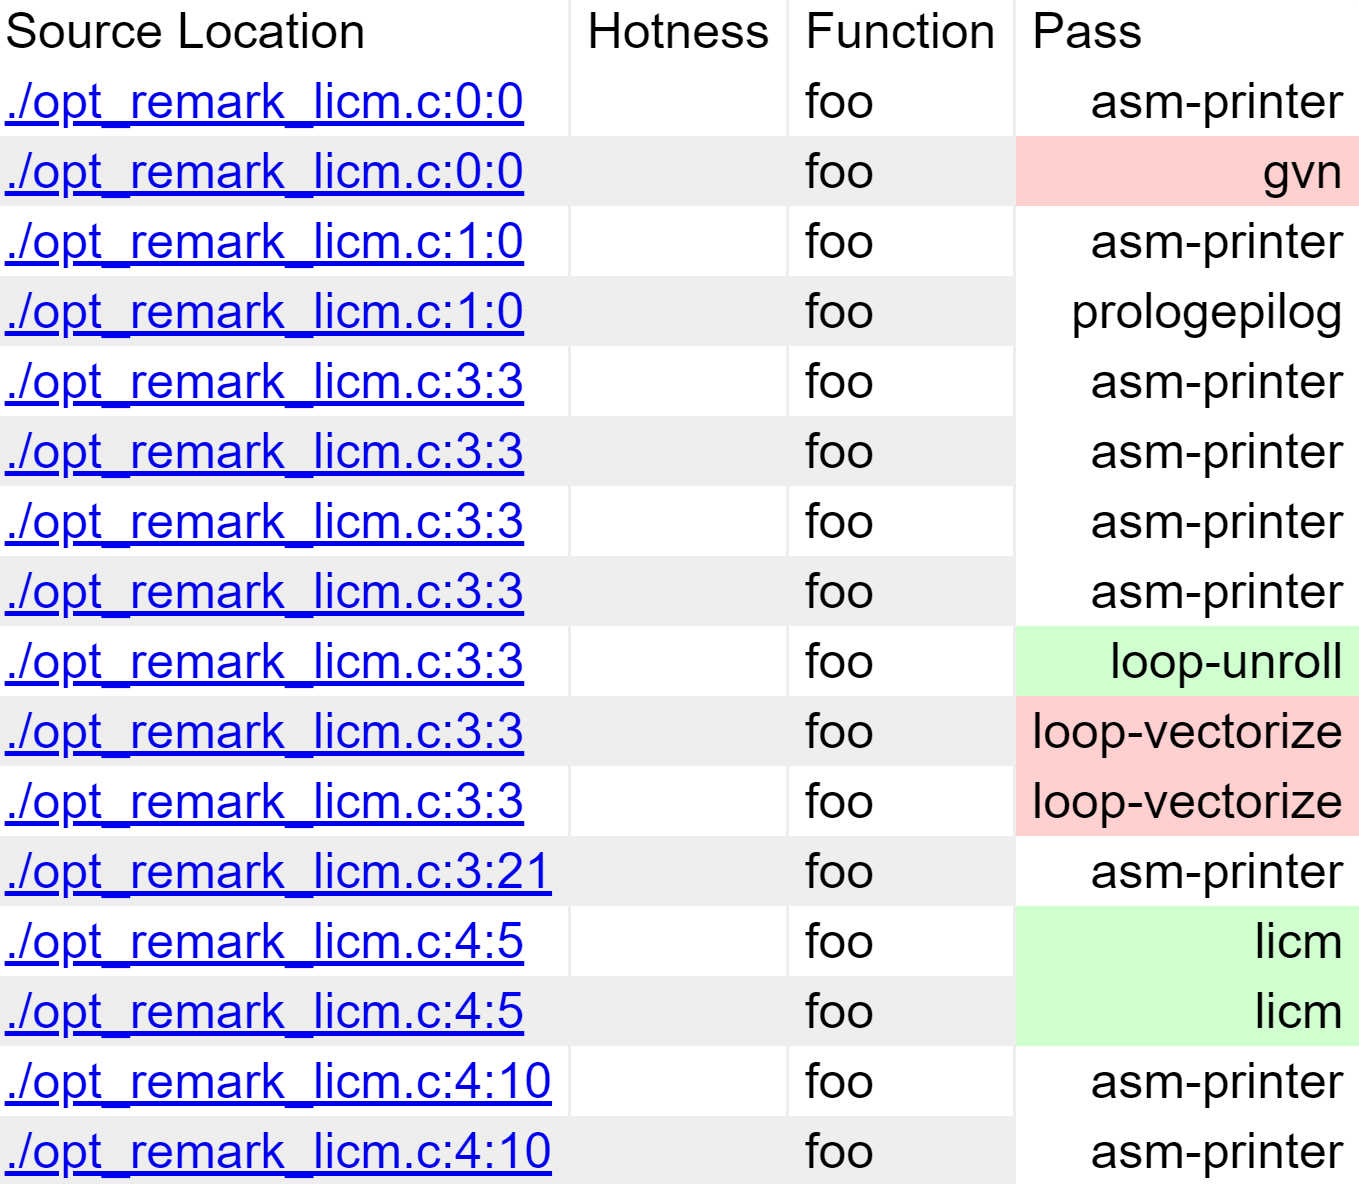
\includegraphics[width=0.7\textwidth]{content/3/chapter11/images/1.png}\\
图11.1 - Web页面的优化注释与源文件的结合
\end{center}

我们对其中的两列特别感兴趣:\textbf{Source Location}和\textbf{Pass}。后一列显示了Pass的名称和优化注释的类型——以红色、绿色和白色呈现的\texttt{Missed}、\texttt{Passed}或\texttt{Analyzed},分别附加在\textbf{Source Location}列的给定行上。

如果点击源位置列中的链接,这将导航到这样一个页面,看起来像这样:

\hspace*{\fill} \\ %插入空行
\begin{center}
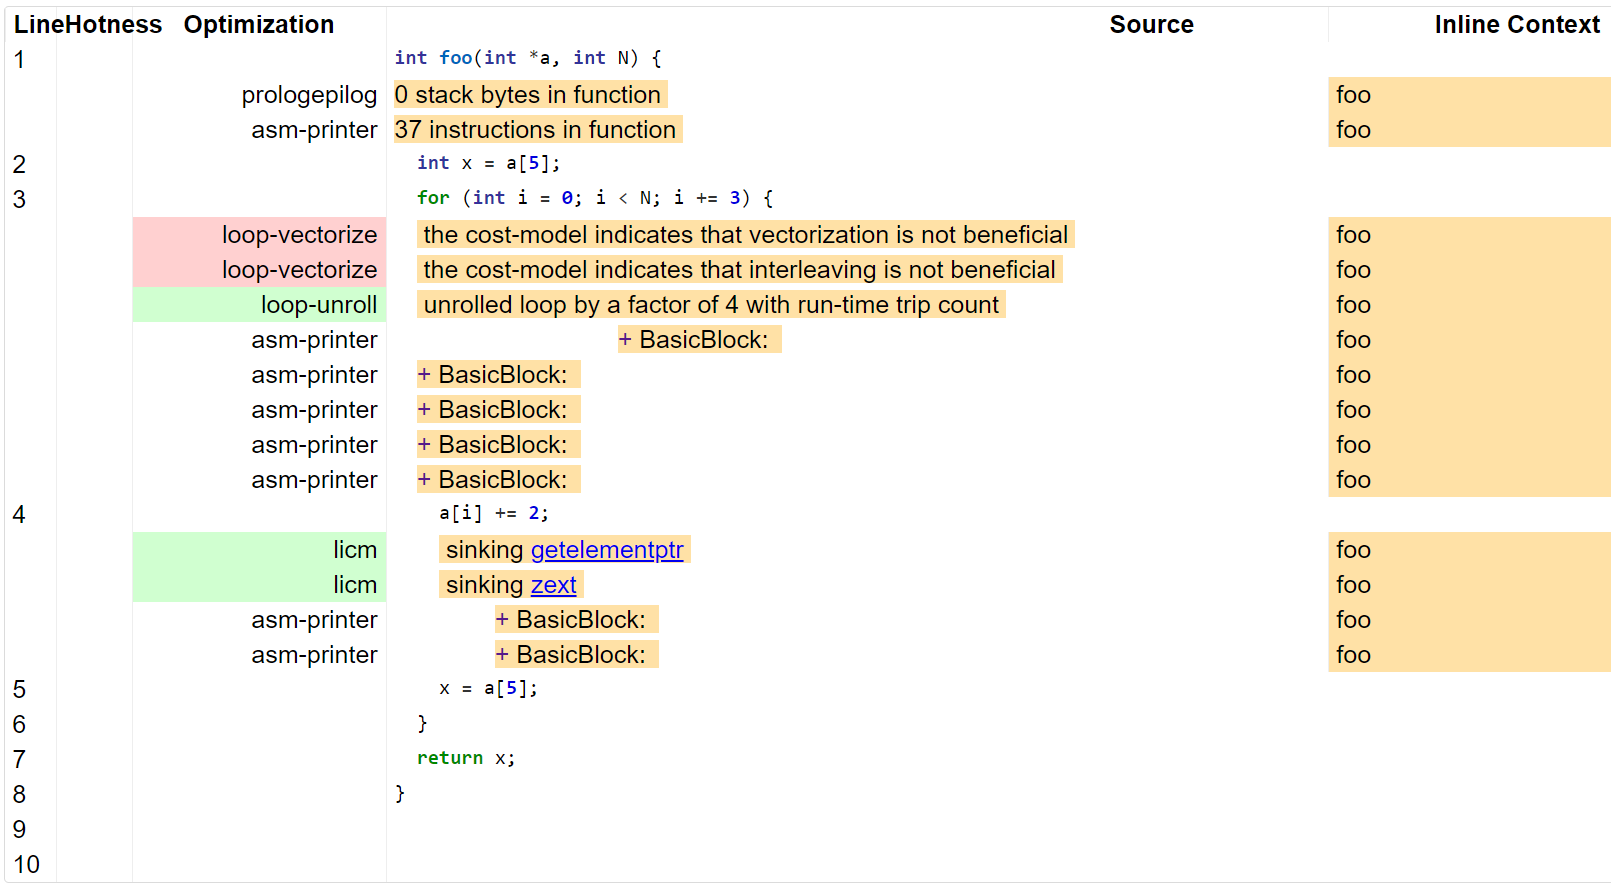
\includegraphics[width=0.9\textwidth]{content/3/chapter11/images/2.png}\\
图11.2 - 优化注释的详细信息
\end{center}

这个页面提供了优化注释细节的一个很好的视图,并与原始源代码行交叉显示。例如,在第3行,\texttt{loop-vectorize} Pass说它不能向量化这个循环,因为它的模型不认为这样做是有益的。

\end{enumerate}

现在,我们已经了解了如何使用优化注释来深入了解优化Pass,这在调试丢失的优化机会或修复编译错误时特别有用。

下一节中,我们将了解一些有用的技能来分析LLVM的执行时间。





















